\section{KFAC: initial approximation $\tilde{F} \approx F$}
\frame{\tableofcontents[currentsection, hideothersubsections]}

\begin{frame}
\frametitle{KFAC: Initial approximation $\tilde{F} \approx F$}

Recall:
\begin{figure}
    \raggedright
    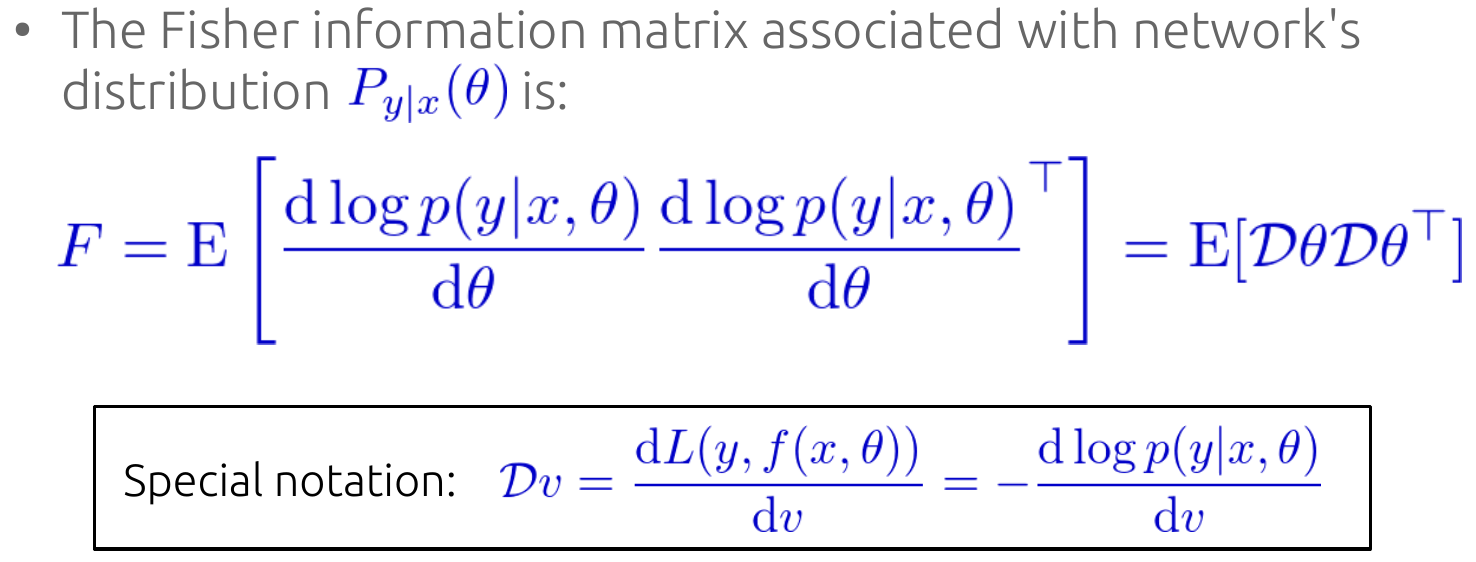
\includegraphics[scale=0.25]{fisher}
\end{figure}

\end{frame}

\begin{frame}
\frametitle{KFAC: Initial approximation $\tilde{F} \approx F$}

\begin{figure}
    \raggedright
    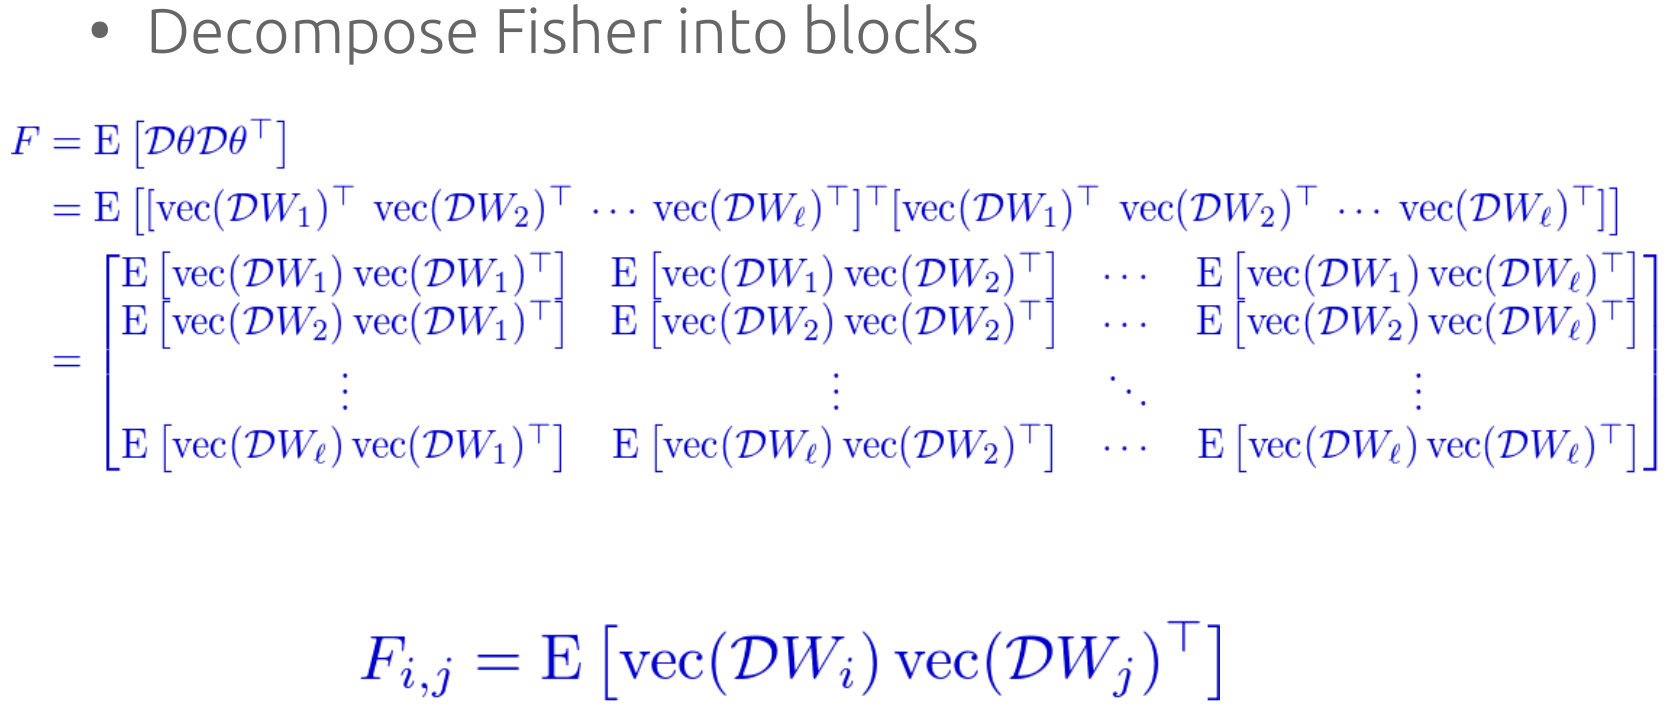
\includegraphics[scale=0.25]{kfac_01}
\end{figure}

$F$ can be viewed as an $\ell$ by $\ell$ block matrix.\\
(blocks correpond to layers)
\end{frame}

\begin{frame}
\frametitle{KFAC: Initial approximation $\tilde{F} \approx F$}

$g_i = \mathcal{D}s_i$ is the derivative of the loss wrt the inputs to units at layer $i$
\begin{figure}
    \raggedright
    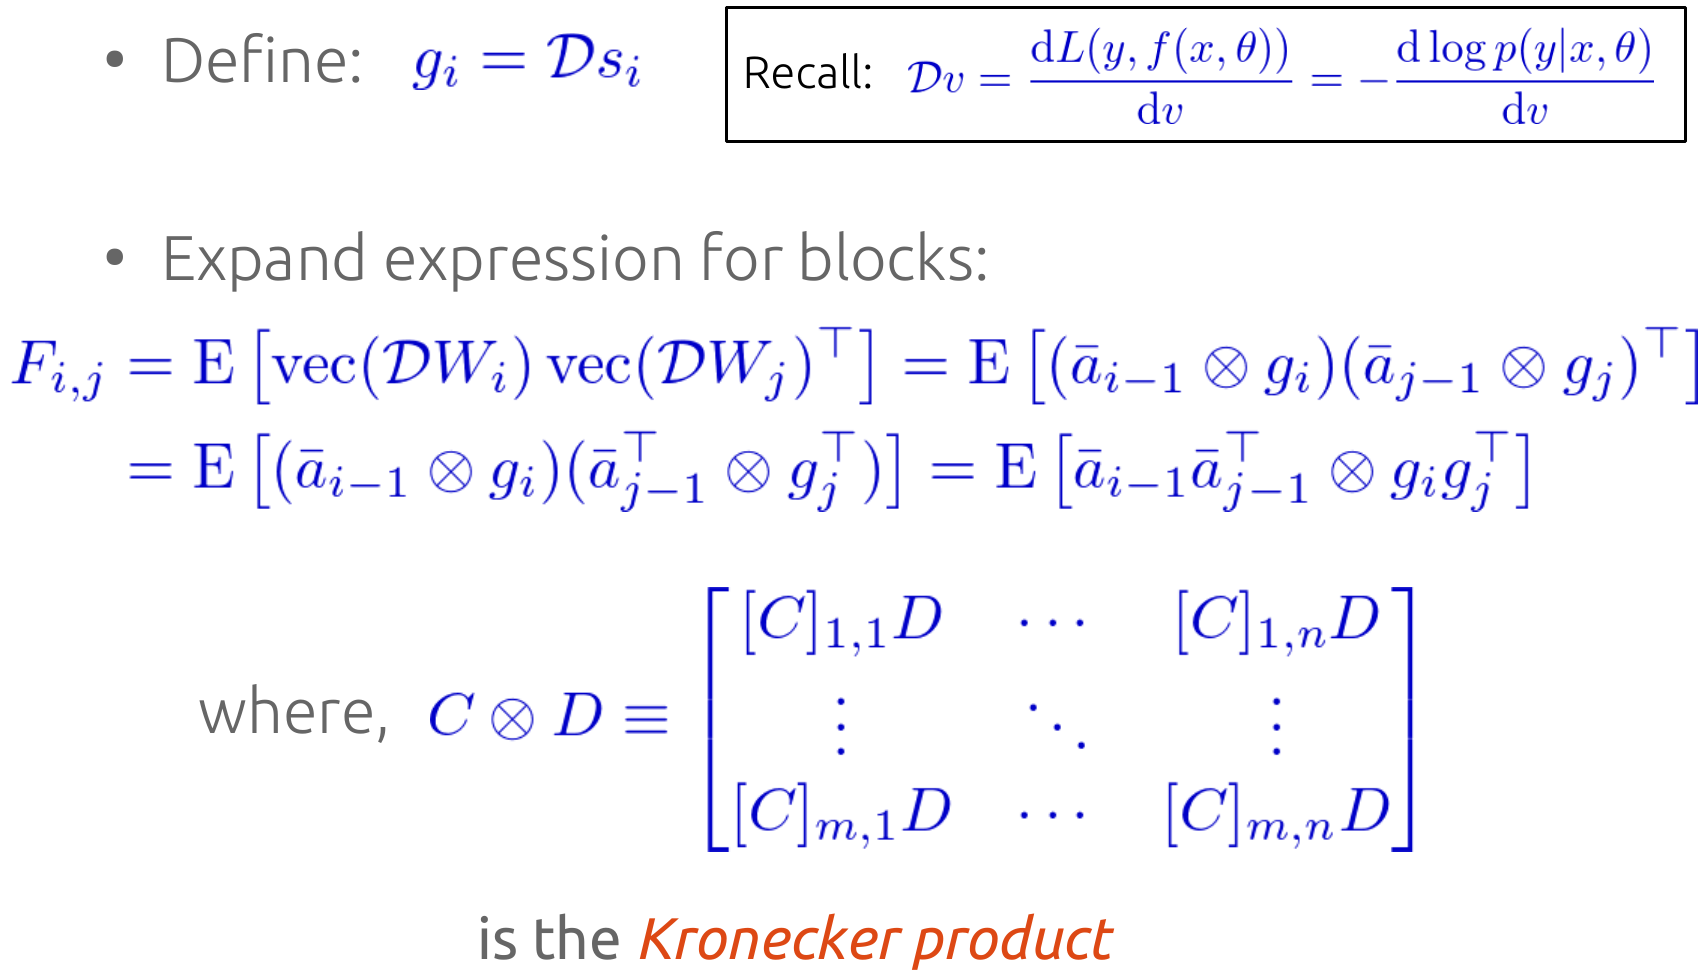
\includegraphics[scale=0.25]{kfac_02}
\end{figure}

Recall: $(A \otimes B)^T = (A^T \otimes B^T)$ and $(A \otimes B) (C \otimes D) = (AC \otimes BD)$
\end{frame}

\begin{frame}
\frametitle{KFAC: Initial approximation $\tilde{F} \approx F$}

\begin{figure}
    \raggedright
    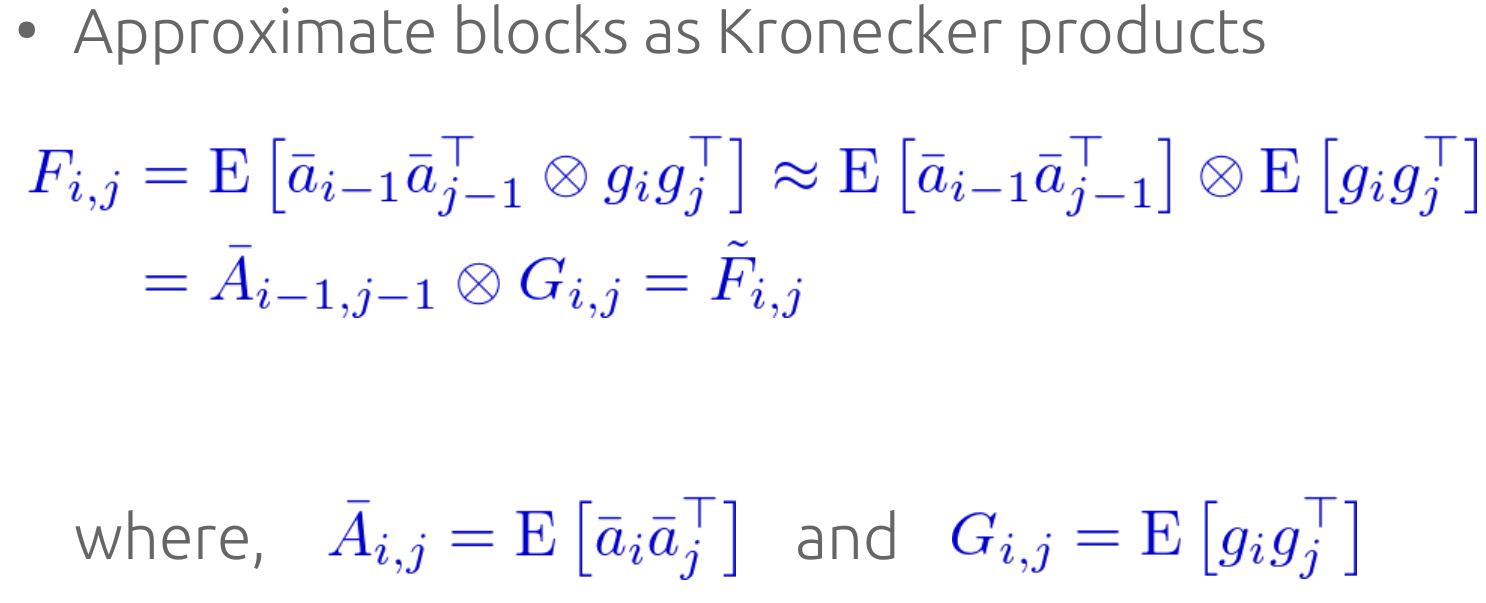
\includegraphics[scale=0.2]{kfac_03}
\end{figure}

\begin{figure}
    \raggedright
    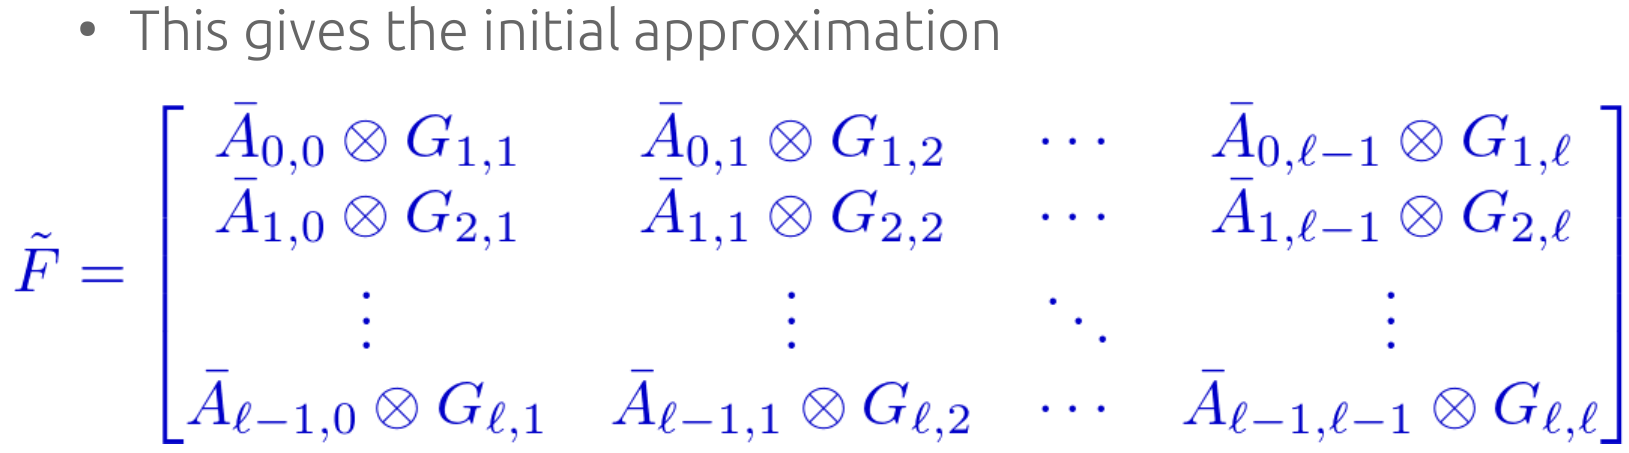
\includegraphics[scale=0.2]{kfac_04}
\end{figure}

$\tilde{F}$ is indeed a major approximation because\\
the expectation of a Kronecker product is, in general, NOT
equal to the Kronecker product of expectations

\end{frame}

\begin{frame}
\frametitle{KFAC: Initial approximation $\tilde{F} \approx F$}
Comparing the exact $F$ vs its approximate $\tilde{F}$
\begin{figure}
    \centering
    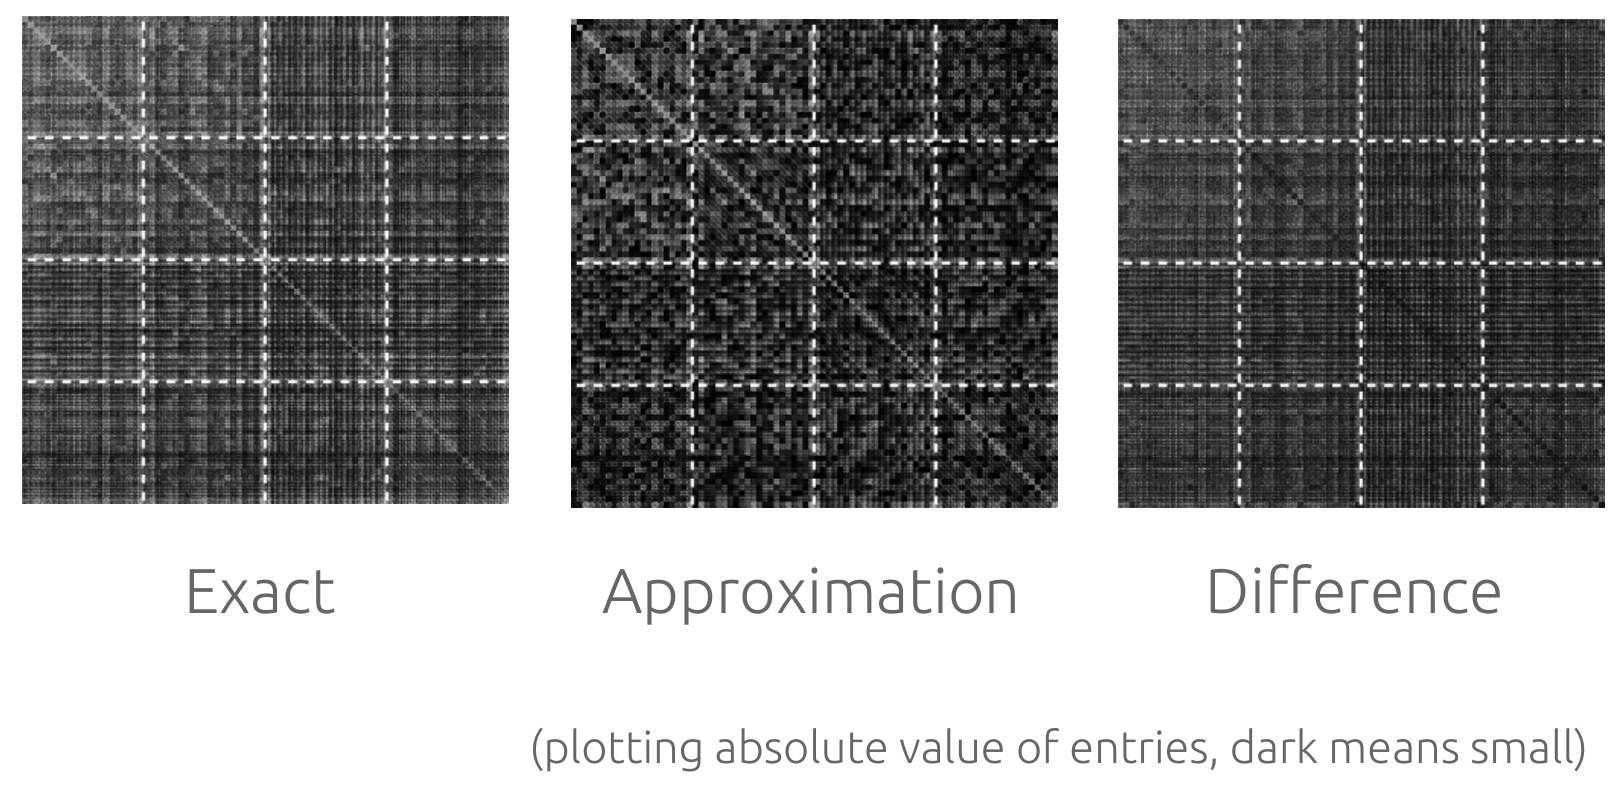
\includegraphics[scale=0.275]{kfac_05}
\end{figure}

\end{frame}

\begin{frame}
\frametitle{KFAC: Initial approximation $\tilde{F} \approx F$}
Recall:
\begin{figure}
    \raggedright
    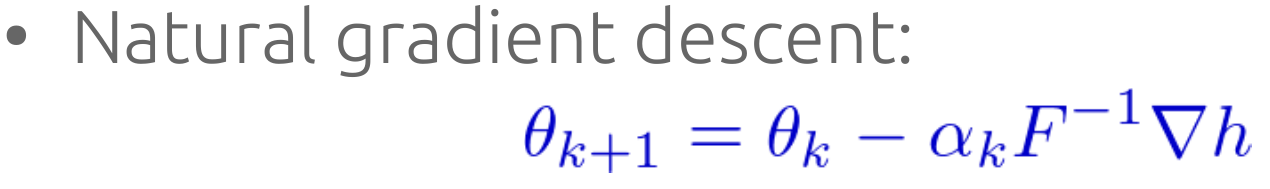
\includegraphics[scale=0.2]{natgrad}
\end{figure}

We already have $\tilde{F} \approx F$, then: \\
how to \textbf{efficiently} compute $\tilde{F}^{-1}$ or its product, $\tilde{F}^{-1}\nabla h$?
\end{frame}

\begin{frame}
\frametitle{KFAC: Initial approximation $\tilde{F} \approx F$}
Structure in the inverse Fisher:
\begin{figure}
    \centering
    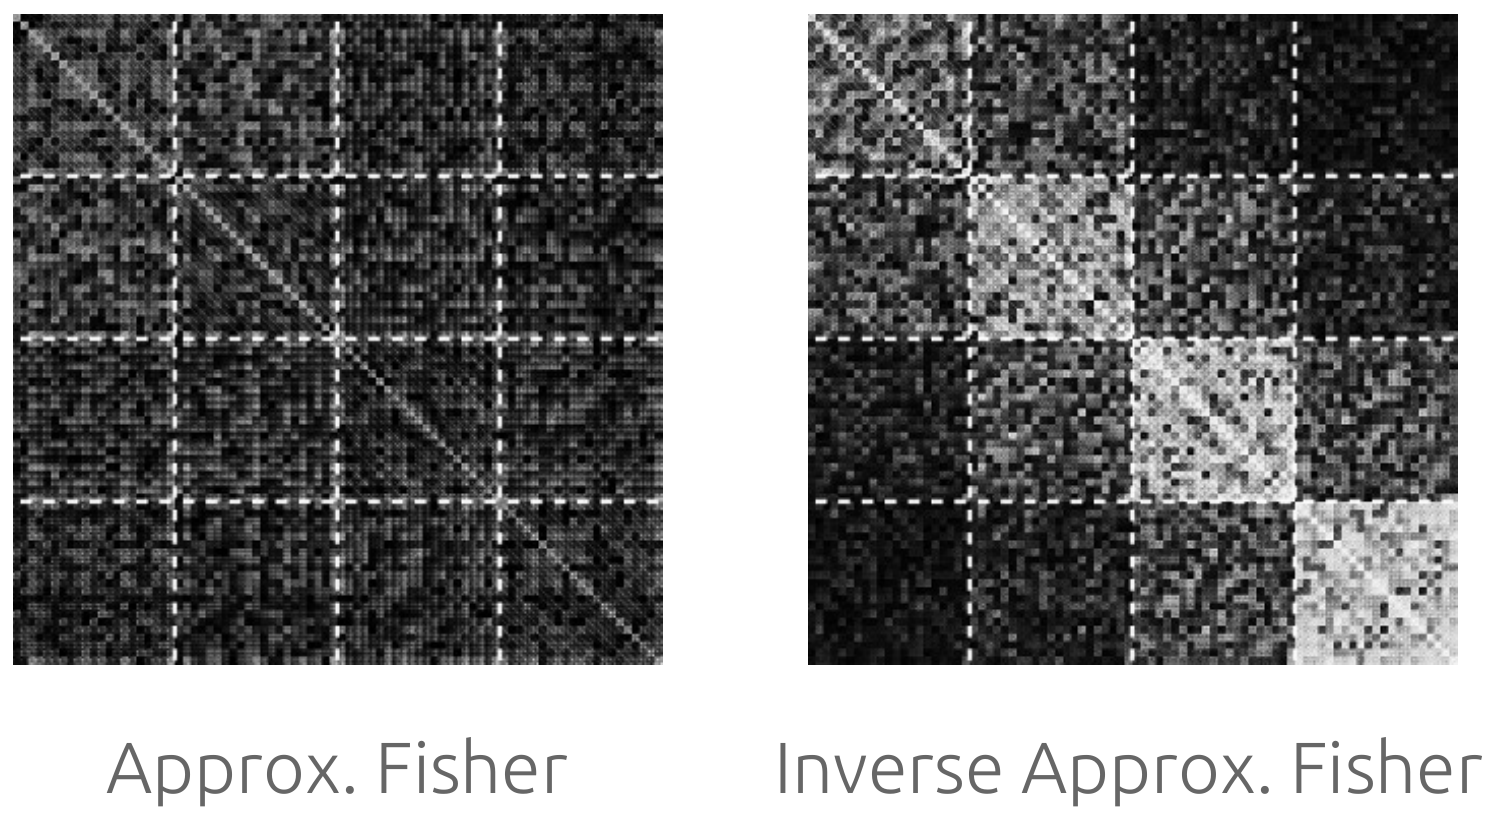
\includegraphics[scale=0.2]{kfac_06}
\end{figure}
(plotting absolute value of entries, dark means small)
\end{frame}

\begin{frame}
\frametitle{KFAC: Initial approximation $\tilde{F} \approx F$}
Based on Structured Inverses (Pourahmadi, 2011):
\begin{figure}
    \raggedright
    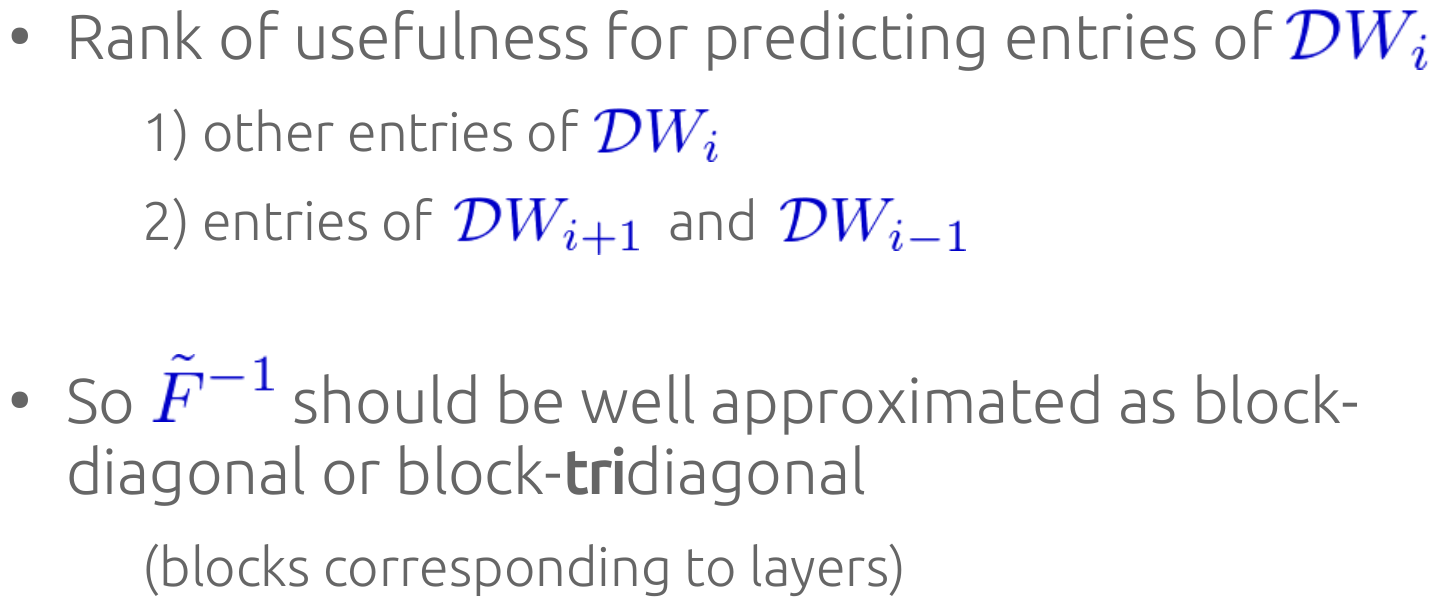
\includegraphics[scale=0.275]{kfac_07}
\end{figure}
\end{frame}
